\documentclass[tikz,border=10pt]{standalone}
% Shared look for every TikZ diagram. Load with % Shared look for every TikZ diagram. Load with % Shared look for every TikZ diagram. Load with \input{../../tools/tikz-style.tex}
\usepackage[T1]{fontenc}
\usepackage{lmodern}
\renewcommand{\sfdefault}{lmr}  % diagrams use the same serif as the text
\usetikzlibrary{arrows.meta, positioning, shapes.geometric, calc, fit, backgrounds}
\definecolor{cblue}{HTML}{4C78A8}
\definecolor{corange}{HTML}{F58518}
\definecolor{cgreen}{HTML}{54A24B}
\definecolor{cred}{HTML}{E45756}
\definecolor{cpurple}{HTML}{B279A2}
\definecolor{cgrey}{HTML}{6B6B6B}
\tikzset{
  every picture/.style={font=\sffamily, line width=1.2pt},
  box/.style={draw=#1, fill=#1!12, rounded corners=4pt, align=center, inner sep=7pt, minimum height=1.1cm},
  box/.default=cgrey,
  arrow/.style={-{Stealth[length=3mm]}, draw=cgrey, line width=1.4pt},
  title/.style={font=\sffamily\bfseries\Large},
  note/.style={font=\sffamily\small, text=cgrey, align=center},
}
\AtBeginDocument{\hyphenpenalty=10000 \exhyphenpenalty=10000}

\usepackage[T1]{fontenc}
\usepackage{lmodern}
\renewcommand{\sfdefault}{lmr}  % diagrams use the same serif as the text
\usetikzlibrary{arrows.meta, positioning, shapes.geometric, calc, fit, backgrounds}
\definecolor{cblue}{HTML}{4C78A8}
\definecolor{corange}{HTML}{F58518}
\definecolor{cgreen}{HTML}{54A24B}
\definecolor{cred}{HTML}{E45756}
\definecolor{cpurple}{HTML}{B279A2}
\definecolor{cgrey}{HTML}{6B6B6B}
\tikzset{
  every picture/.style={font=\sffamily, line width=1.2pt},
  box/.style={draw=#1, fill=#1!12, rounded corners=4pt, align=center, inner sep=7pt, minimum height=1.1cm},
  box/.default=cgrey,
  arrow/.style={-{Stealth[length=3mm]}, draw=cgrey, line width=1.4pt},
  title/.style={font=\sffamily\bfseries\Large},
  note/.style={font=\sffamily\small, text=cgrey, align=center},
}
\AtBeginDocument{\hyphenpenalty=10000 \exhyphenpenalty=10000}

\usepackage[T1]{fontenc}
\usepackage{lmodern}
\renewcommand{\sfdefault}{lmr}  % diagrams use the same serif as the text
\usetikzlibrary{arrows.meta, positioning, shapes.geometric, calc, fit, backgrounds}
\definecolor{cblue}{HTML}{4C78A8}
\definecolor{corange}{HTML}{F58518}
\definecolor{cgreen}{HTML}{54A24B}
\definecolor{cred}{HTML}{E45756}
\definecolor{cpurple}{HTML}{B279A2}
\definecolor{cgrey}{HTML}{6B6B6B}
\tikzset{
  every picture/.style={font=\sffamily, line width=1.2pt},
  box/.style={draw=#1, fill=#1!12, rounded corners=4pt, align=center, inner sep=7pt, minimum height=1.1cm},
  box/.default=cgrey,
  arrow/.style={-{Stealth[length=3mm]}, draw=cgrey, line width=1.4pt},
  title/.style={font=\sffamily\bfseries\Large},
  note/.style={font=\sffamily\small, text=cgrey, align=center},
}
\AtBeginDocument{\hyphenpenalty=10000 \exhyphenpenalty=10000}

\begin{document}
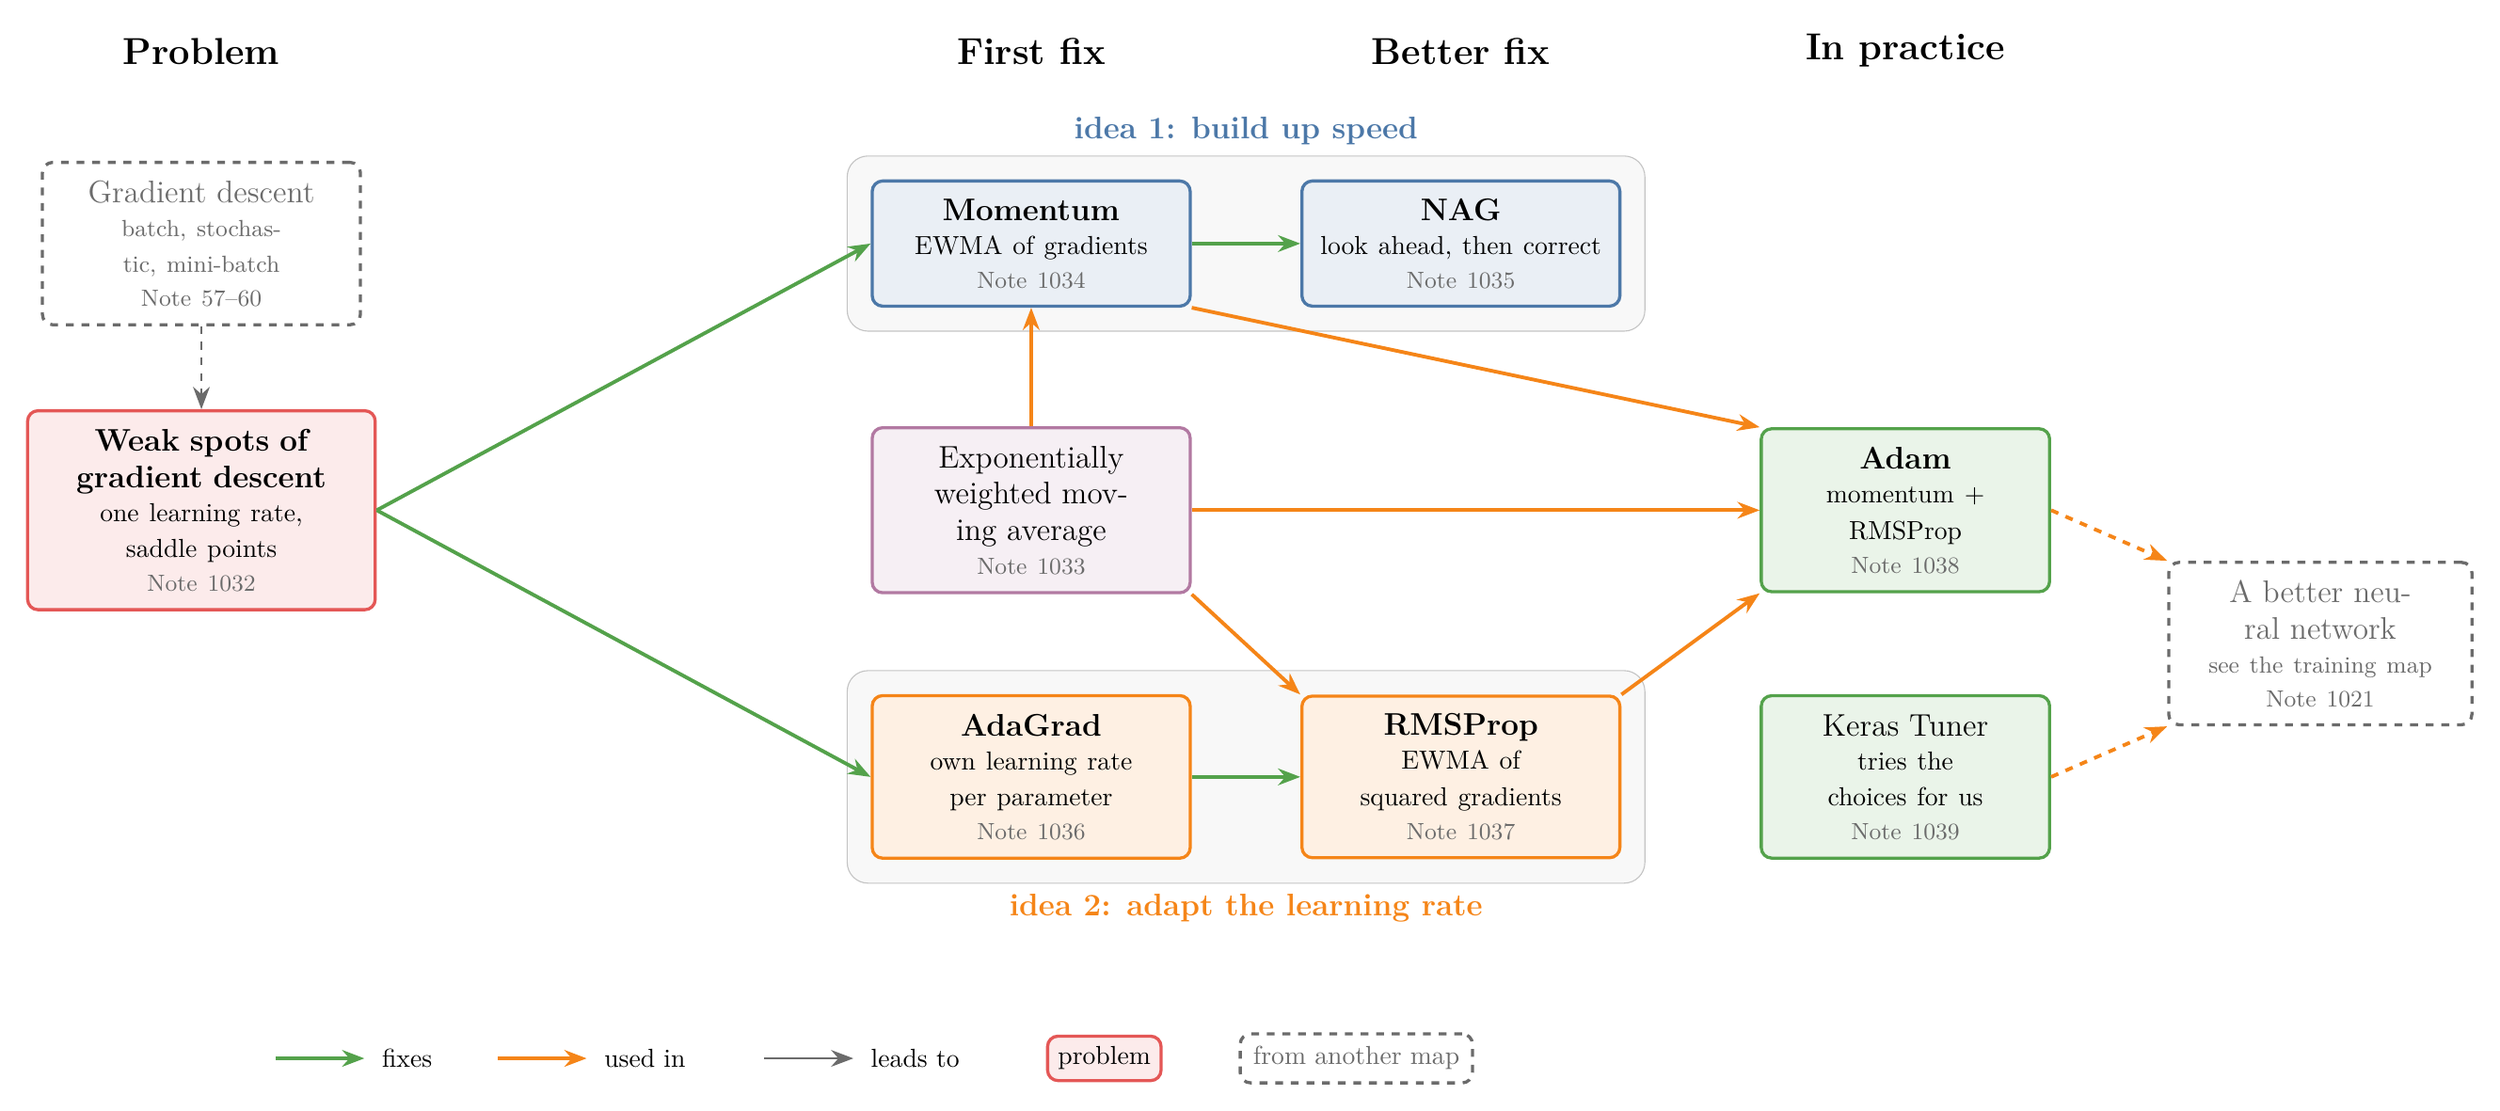
\begin{tikzpicture}[
    every node/.append style={font=\sffamily\large},
    con/.style={box=cblue, text width=4.0cm},
    prob/.style={box=cred, text width=4.0cm},
    prev/.style={draw=cgrey, dashed, rounded corners=4pt, align=center, inner sep=7pt, text=cgrey, text width=3.8cm, minimum height=1.1cm},
    group/.style={draw=cgrey!40, fill=cgrey!5, rounded corners=8pt, inner sep=9pt},
    kind/.style={arrow, draw=cgrey, line width=1pt},
    needs/.style={arrow, draw=cpurple},
    fixes/.style={arrow, draw=cgreen},
    usedin/.style={arrow, draw=corange},
  ]
  \newcommand{\nt}[1]{\\[-1pt]{\small\color{cgrey}Note #1}}
  \newcommand{\sub}[1]{\\[-1pt]{\normalsize #1}}
  \node[title] at (0,6.2) {Problem};
  \node[title] at (11.2,6.2) {First fix};
  \node[title] at (17.0,6.2) {Better fix};
  \node[title] at (23.0,6.2) {In practice};

  % problem
  \node[prev] (gd) at (0,3.6) {Gradient descent\\[-1pt]{\small batch, stochastic, mini-batch}\nt{57--60}};
  \node[prob, text width=4.2cm] (weak) at (0,0) {\textbf{Weak spots of gradient descent}\sub{one learning rate, saddle points}\nt{1032}};
  \draw[kind, dashed] (gd) -- (weak);

  % idea 1: speed
  \node[con, text width=3.8cm] (mom) at (11.2,3.6) {\textbf{Momentum}\sub{EWMA of gradients}\nt{1034}};
  \node[con, text width=3.8cm] (nag) at (17.0,3.6) {\textbf{NAG}\sub{look ahead, then correct}\nt{1035}};
  % idea 2: adaptive learning rate
  \node[box=corange, text width=3.8cm] (ada) at (11.2,-3.6) {\textbf{AdaGrad}\sub{own learning rate per parameter}\nt{1036}};
  \node[box=corange, text width=3.8cm] (rms) at (17.0,-3.6) {\textbf{RMSProp}\sub{EWMA of squared gradients}\nt{1037}};
  \begin{scope}[on background layer]
    \node[group, fit=(mom) (nag)] (g1) {};
    \node[group, fit=(ada) (rms)] (g2) {};
  \end{scope}
  \node[font=\sffamily\bfseries\large, text=cblue, anchor=south] at (g1.north) {idea 1: build up speed};
  \node[font=\sffamily\bfseries\large, text=corange, anchor=north] at (g2.south) {idea 2: adapt the learning rate};

  % tool
  \node[box=cpurple, text width=3.8cm] (ewma) at (11.2,0) {Exponentially weighted moving average\nt{1033}};

  % goal
  \node[box=cgreen, text width=3.4cm, minimum height=2.2cm] (adam) at (23.0,0) {\textbf{Adam}\sub{momentum + RMSProp}\nt{1038}};
  \node[box=cgreen, text width=3.4cm] (tuner) at (23.0,-3.6) {Keras Tuner\sub{tries the choices for us}\nt{1039}};
  \node[prev, text width=3.6cm] (goal) at (28.6,-1.8) {A better neural network\\[-1pt]{\small see the training map}\nt{1021}};

  \draw[fixes] (weak.east) -- (mom.west);
  \draw[fixes] (weak.east) -- (ada.west);
  \draw[fixes] (mom) -- (nag);
  \draw[fixes] (ada) -- (rms);
  \draw[usedin] (ewma) -- (mom);
  \draw[usedin] (ewma.south east) -- (rms.north west);
  \draw[usedin] (ewma) -- (adam);
  \draw[usedin] (mom.south east) -- (adam.north west);
  \draw[usedin] (rms.north east) -- (adam.south west);
  \draw[usedin, dashed] (adam.east) -- (goal.north west);
  \draw[usedin, dashed] (tuner.east) -- (goal.south west);

  % legend
  \begin{scope}[shift={(1.0,-7.4)}, every node/.style={font=\sffamily, anchor=west}]
    \draw[fixes] (0,0) -- (1.2,0);      \node at (1.3,0) {fixes};
    \draw[usedin] (3.0,0) -- (4.2,0);   \node at (4.3,0) {used in};
    \draw[kind] (6.6,0) -- (7.8,0);     \node at (7.9,0) {leads to};
    \node[box=cred, minimum height=0.6cm, inner sep=4pt, anchor=west] at (10.4,0) {problem};
    \node[draw=cgrey, dashed, rounded corners=4pt, inner sep=5pt, text=cgrey, anchor=west] at (13.0,0) {from another map};
  \end{scope}
\end{tikzpicture}
\end{document}
